\documentclass[12pt]{article}
\usepackage[utf8]{inputenc}
\usepackage{float}
\usepackage{amsmath}
\usepackage{indentfirst}

\usepackage[hmargin=3cm,vmargin=6.0cm]{geometry}
%\topmargin=0cm
\topmargin=-2cm
\addtolength{\textheight}{6.5cm}
\addtolength{\textwidth}{2.0cm}
%\setlength{\leftmargin}{-5cm}
\setlength{\oddsidemargin}{0.0cm}
\setlength{\evensidemargin}{0.0cm}

%misc libraries goes here
\usepackage{tikz}
\usetikzlibrary{automata,positioning}

\begin{document}

\section*{Student Information } 
%Write your full name and id number between the colon and newline
%Put one empty space character after colon and before newline
Full Name :  Ugur Duzel \par
Id Number :  2171569 \\

% Write your answers below the section tags
\section*{Answer 1}

\subsection*{a.}
There can be infinitely many digits in the decimal part of the rational numbers inside $(-1,0)$. It is obvious that the rational numbers inside $(-1,0)$ are infinitely many. The question is that rather it is countable or uncountable.
Assume that $R_{(-1,0)}$ is countably infinite. Any number in $R_{(-1,0)}$ must be in the following form. 
$$-0.d_1d_2d_3...d_i\quad d_i\in \{0,1,2,\ ...,9\}$$
We can enumarate elements in $R_{(-1,0)}$,
$$-0.a_{11}a_{12}a_{13}a_{14}... \quad \leftarrow 1^{st}\ number$$
$$-0.a_{21}a_{22}a_{23}a_{24}... \quad \leftarrow 2^{nd}\ number$$
$$-0.a_{31}a_{32}a_{33}a_{34}... \quad \leftarrow 3^{rd}\ number$$
$$-0.a_{41}a_{42}a_{43}a_{44}... \quad \leftarrow 4^{th}\ number$$
$$...$$
$$-0.a_{i1}a_{i2}a_{i3}a_{i4}... \quad \leftarrow i^{th}\ number$$
$a_{ij}$ is the $j^{th}$ digit of $i^{th}$ number $\in \{0,1,2,\ ...,9\}$. \\ \par
If we are able to compose a number that is not in this listing, then contradiction occurs. \\ 
Let's call the number we are composing $b$ such that, 
$$b=-0.b_1b_2b_3...b_i$$
\[
  b_i =
  \begin{cases}
                                   1 & \text{if $a_{ii}=9$} \\
                                   9-a_{ii} & \text{otherwise} 
  \end{cases}
\]
$b$ is different than $1^{st}$ number in the list in $1^{st}$ digit. \\
$b$ is different than $2^{nd}$ number in the list in $2^{st}$ digit. \\
...\\
$b$ is different than $i^{th}$ number in the list in $i^{th}$ digit. \\
The number $b$ does not appear in the list. This leads to contradiction. \\ \par
Therefore, the assumption - countably infinite - is wrong.  The set of rational numbers inside the $(-1,0)$ is infinite and uncountable.


\subsection*{b.}  
First of all we know by the theorem that a language is regular if and only if it can be recognized by a Finite Automaton. Now we should constructively prove the following, \\
Any finite language is regular. \\
Proof: Let L $\subseteq \Sigma ^*$ be a finite language.
$$L=\emptyset \ \text{or}\ L=\{w_1,w_2,...w_n\}\ \text{for}\ n>0$$
We can construct the finite automata $M$ such that
$$L(M)=L=\{w_1\}\cup \{w_2\}\cup ... \{w_n\} = L_{w_1}\cup L_{w_2}\cup ... L_{w_n}$$ 
as $M= M_{\emptyset}\cup M_{w_1}\cup M_{w_2}\cup ... M_{w_n}$. Since we are able to construct a finite automata $M$, we can say that $L(M)=L$ is regular. \par
In the question we are given a finite language $L$ over the unary alpahabet $\Sigma=\{a\}$, so given language L is regular.
By the theorem, we know that the languages accepted by a finite automata, also regular languages, are closed under concatenation and kleene star operations. Therefore, $L^+=LL^*$ is regular. \par
$L^+$ cannot be both regular and not regular. So, $D=\emptyset$. The empty set is finite and countable. 


\subsection*{c.}
Given an alphabet $\Sigma$, regular expressions over $\Sigma$ are all strings over the alphabet 
$\Sigma \cup \{(,),\emptyset,\cup,^*\}$. 
By the theorem, we know that for any non-empty finite set A, the set $A^*$ is countably infinite, i.e. $|A^*|=\aleph$. \par
The set $R$ of regular expressions over an alphabet $\Sigma$ is countably infinite. To prove it, the set $\Sigma \cup \{(,),\emptyset,\cup,^*\}$ is non-empty and finite, so the set $(\Sigma \cup \{(,),\emptyset,\cup,^*\})^*$ is countably infinite and by the definition
$$R\subseteq (\Sigma \cup \{(,),\emptyset,\cup,^*\})^*$$ 
hence $|R|\leq \aleph$. The set $R$ of regular expressions is countably infinite. \\
The class of regular languages over an alphabet $\Sigma$ is defined to consist of all languages $L$ such that $L=L(r)$ for some regular expression $r$ over $\Sigma$. This means that the set of regular languages is countably infinite as well. \par
We know that the set of all languages over an alphabet is uncountable and infinite. In the question we are given the set of all languages which cannot be recognized by any Finite Automaton. Because of the known theorem, a language is regular if and only if it can be recognized by a Finite Automaton, the question asks for the set of all languages that is not regular. Let's call this set $R'$. $R'$ can be represented as $R'=2^{\Sigma ^*}  -\ R$ \\
The difference of an uncountably infinite set and a countably infinite set results in uncountably infinite set. So the answer is uncountable and infinite.
 



\section*{Answer 2}

\subsection*{a.}

\textbf{\underline{Start state}: }$q_0$

\begin{center}
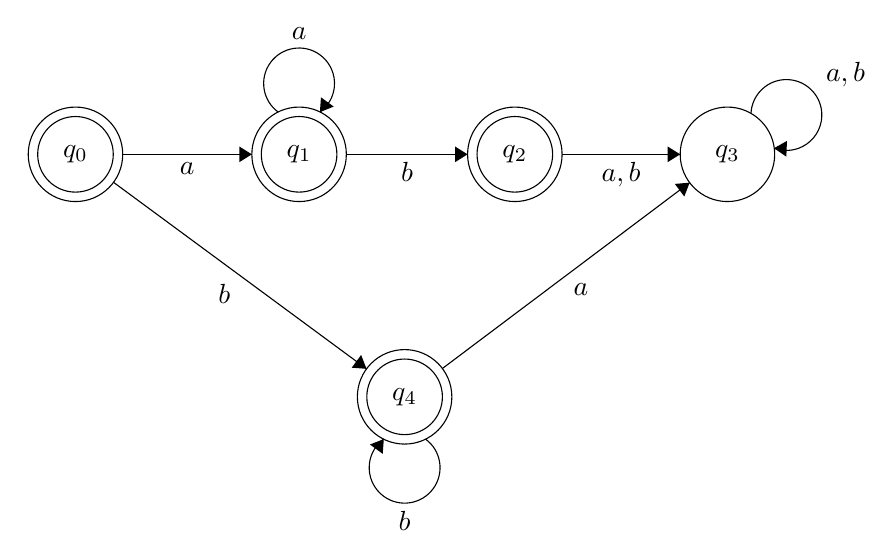
\begin{tikzpicture}[scale=0.2]
\tikzstyle{every node}+=[inner sep=0pt]
\draw [black] (19.2,-12.8) circle (3);
\draw (19.2,-12.8) node {$q_0$};
\draw [black] (19.2,-12.8) circle (2.4);
\draw [black] (33.4,-12.8) circle (3);
\draw (33.4,-12.8) node {$q_1$};
\draw [black] (33.4,-12.8) circle (2.4);
\draw [black] (47.1,-12.8) circle (3);
\draw (47.1,-12.8) node {$q_2$};
\draw [black] (47.1,-12.8) circle (2.4);
\draw [black] (60.6,-12.8) circle (3);
\draw (60.6,-12.8) node {$q_3$};
\draw [black] (40.1,-28.2) circle (3);
\draw (40.1,-28.2) node {$q_4$};
\draw [black] (40.1,-28.2) circle (2.4);
\draw [black] (21.62,-14.58) -- (37.68,-26.42);
\fill [black] (37.68,-26.42) -- (37.34,-25.54) -- (36.74,-26.35);
\draw (28.65,-21) node [below] {$b$};
\draw [black] (22.2,-12.8) -- (30.4,-12.8);
\fill [black] (30.4,-12.8) -- (29.6,-12.3) -- (29.6,-13.3);
\draw (26.3,-13.3) node [below] {$a$};
\draw [black] (36.4,-12.8) -- (44.1,-12.8);
\fill [black] (44.1,-12.8) -- (43.3,-12.3) -- (43.3,-13.3);
\draw (40.25,-13.3) node [below] {$b$};
\draw [black] (50.1,-12.8) -- (57.6,-12.8);
\fill [black] (57.6,-12.8) -- (56.8,-12.3) -- (56.8,-13.3);
\draw (53.85,-13.3) node [below] {$a,b$};
\draw [black] (42.5,-26.4) -- (58.2,-14.6);
\fill [black] (58.2,-14.6) -- (57.26,-14.68) -- (57.86,-15.48);
\draw (51.3,-21) node [below] {$a$};
\draw [black] (32.077,-10.12) arc (234:-54:2.25);
\draw (33.4,-5.55) node [above] {$a$};
\fill [black] (34.72,-10.12) -- (35.6,-9.77) -- (34.79,-9.18);
\draw [black] (62.096,-10.213) arc (177.69007:-110.30993:2.25);
\draw (66.83,-7.72) node [right] {$a,b$};
\fill [black] (63.56,-12.41) -- (64.34,-12.95) -- (64.38,-11.95);
\draw [black] (41.423,-30.88) arc (54:-234:2.25);
\draw (40.1,-35.45) node [below] {$b$};
\fill [black] (38.78,-30.88) -- (37.9,-31.23) -- (38.71,-31.82);
\end{tikzpicture}
\end{center}
\subsection*{b.}

\textbf{\underline{Start state}: }$q_0$

\begin{center}
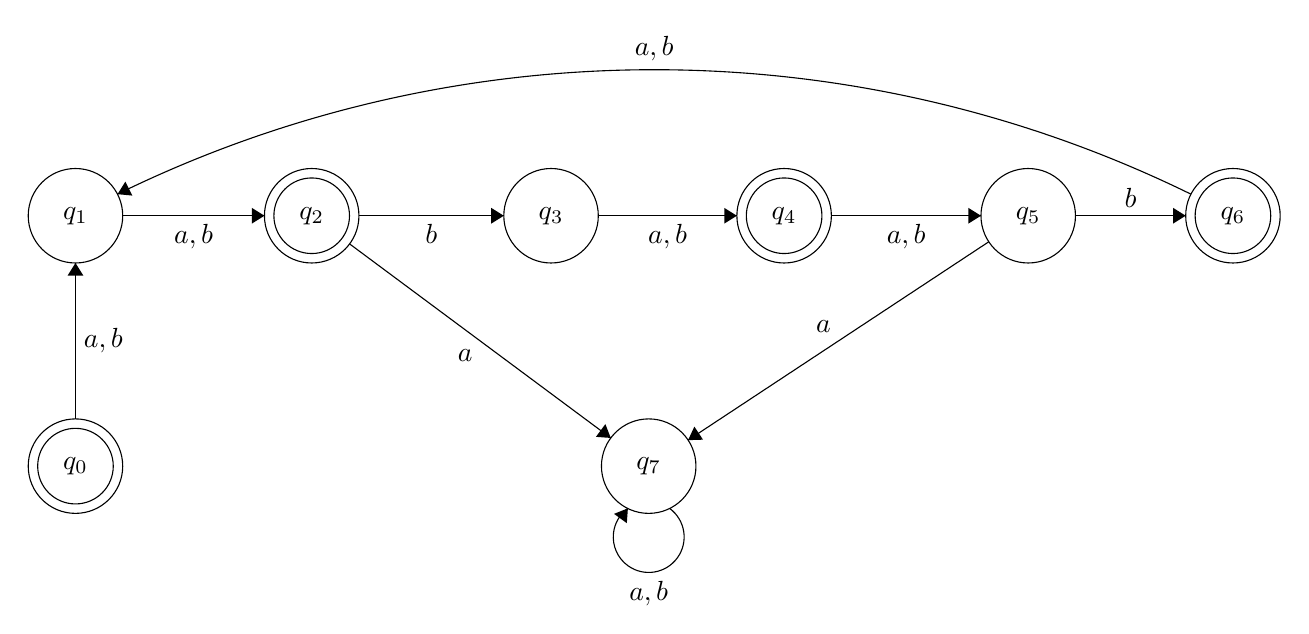
\begin{tikzpicture}[scale=0.2]
\tikzstyle{every node}+=[inner sep=0pt]
\draw [black] (3.4,-32.8) circle (3);
\draw (3.4,-32.8) node {$q_0$};
\draw [black] (3.4,-32.8) circle (2.4);
\draw [black] (3.4,-16.9) circle (3);
\draw (3.4,-16.9) node {$q_1$};
\draw [black] (18.4,-16.9) circle (3);
\draw (18.4,-16.9) node {$q_2$};
\draw [black] (18.4,-16.9) circle (2.4);
\draw [black] (33.6,-16.9) circle (3);
\draw (33.6,-16.9) node {$q_3$};
\draw [black] (48.4,-16.9) circle (3);
\draw (48.4,-16.9) node {$q_4$};
\draw [black] (48.4,-16.9) circle (2.4);
\draw [black] (39.8,-32.8) circle (3);
\draw (39.8,-32.8) node {$q_7$};
\draw [black] (63.9,-16.9) circle (3);
\draw (63.9,-16.9) node {$q_5$};
\draw [black] (76.9,-16.9) circle (3);
\draw (76.9,-16.9) node {$q_6$};
\draw [black] (76.9,-16.9) circle (2.4);
\draw [black] (3.4,-29.8) -- (3.4,-19.9);
\fill [black] (3.4,-19.9) -- (2.9,-20.7) -- (3.9,-20.7);
\draw (3.9,-24.85) node [right] {$a,b$};
\draw [black] (6.4,-16.9) -- (15.4,-16.9);
\fill [black] (15.4,-16.9) -- (14.6,-16.4) -- (14.6,-17.4);
\draw (10.9,-17.4) node [below] {$a,b$};
\draw [black] (21.4,-16.9) -- (30.6,-16.9);
\fill [black] (30.6,-16.9) -- (29.8,-16.4) -- (29.8,-17.4);
\draw (26,-17.4) node [below] {$b$};
\draw [black] (20.81,-18.69) -- (37.39,-31.01);
\fill [black] (37.39,-31.01) -- (37.05,-30.13) -- (36.45,-30.94);
\draw (28.15,-25.35) node [below] {$a$};
\draw [black] (36.6,-16.9) -- (45.4,-16.9);
\fill [black] (45.4,-16.9) -- (44.6,-16.4) -- (44.6,-17.4);
\draw (41,-17.4) node [below] {$a,b$};
\draw [black] (51.4,-16.9) -- (60.9,-16.9);
\fill [black] (60.9,-16.9) -- (60.1,-16.4) -- (60.1,-17.4);
\draw (56.15,-17.4) node [below] {$a,b$};
\draw [black] (66.9,-16.9) -- (73.9,-16.9);
\fill [black] (73.9,-16.9) -- (73.1,-16.4) -- (73.1,-17.4);
\draw (70.4,-16.4) node [above] {$b$};
\draw [black] (41.123,-35.48) arc (54:-234:2.25);
\draw (39.8,-40.05) node [below] {$a,b$};
\fill [black] (38.48,-35.48) -- (37.6,-35.83) -- (38.41,-36.42);
\draw [black] (61.4,-18.55) -- (42.3,-31.15);
\fill [black] (42.3,-31.15) -- (43.25,-31.12) -- (42.7,-30.29);
\draw (50.9,-24.35) node [above] {$a$};
\draw [black] (6.067,-15.528) arc (116.11479:63.88521:77.43);
\fill [black] (6.07,-15.53) -- (7.01,-15.62) -- (6.57,-14.73);
\draw (40.15,-7.12) node [above] {$a,b$};
\end{tikzpicture}
\end{center}
\vspace{2cm}
\subsection*{c.}

\textbf{\underline{Start state}: }$q_0$

\begin{center}
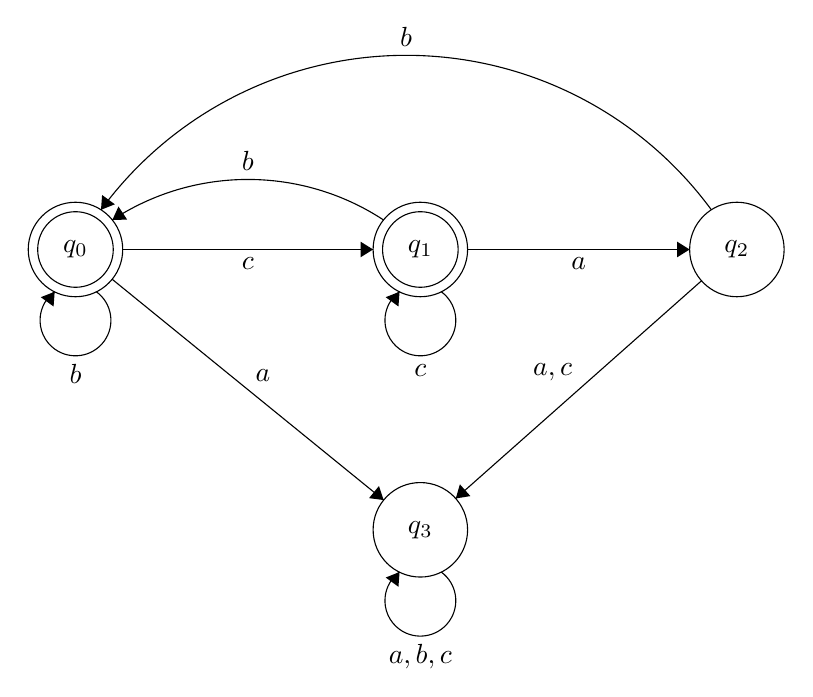
\begin{tikzpicture}[scale=0.2]
\tikzstyle{every node}+=[inner sep=0pt]
\draw [black] (18.5,-18.1) circle (3);
\draw (18.5,-18.1) node {$q_0$};
\draw [black] (18.5,-18.1) circle (2.4);
\draw [black] (40.4,-18.1) circle (3);
\draw (40.4,-18.1) node {$q_1$};
\draw [black] (40.4,-18.1) circle (2.4);
\draw [black] (60.5,-18.1) circle (3);
\draw (60.5,-18.1) node {$q_2$};
\draw [black] (40.4,-35.9) circle (3);
\draw (40.4,-35.9) node {$q_3$};
\draw [black] (21.5,-18.1) -- (37.4,-18.1);
\fill [black] (37.4,-18.1) -- (36.6,-17.6) -- (36.6,-18.6);
\draw (29.45,-18.6) node [below] {$c$};
\draw [black] (58.25,-20.09) -- (42.65,-33.91);
\fill [black] (42.65,-33.91) -- (43.58,-33.76) -- (42.91,-33.01);
\draw (48.8,-26.51) node [above] {$a,c$};
\draw [black] (20.836,-16.225) arc (123.26747:56.73253:15.703);
\fill [black] (20.84,-16.23) -- (21.78,-16.2) -- (21.23,-15.37);
\draw (29.45,-13.15) node [above] {$b$};
\draw [black] (20.121,-15.578) arc (143.69157:36.30843:24.048);
\fill [black] (20.12,-15.58) -- (21,-15.23) -- (20.19,-14.64);
\draw (39.5,-5.27) node [above] {$b$};
\draw [black] (41.723,-38.58) arc (54:-234:2.25);
\draw (40.4,-43.15) node [below] {$a,b,c$};
\fill [black] (39.08,-38.58) -- (38.2,-38.93) -- (39.01,-39.52);
\draw [black] (20.83,-19.99) -- (38.07,-34.01);
\fill [black] (38.07,-34.01) -- (37.77,-33.12) -- (37.14,-33.89);
\draw (30.4,-26.51) node [above] {$a$};
\draw [black] (19.823,-20.78) arc (54:-234:2.25);
\draw (18.5,-25.35) node [below] {$b$};
\fill [black] (17.18,-20.78) -- (16.3,-21.13) -- (17.11,-21.72);
\draw [black] (41.723,-20.78) arc (54:-234:2.25);
\draw (40.4,-25.35) node [below] {$c$};
\fill [black] (39.08,-20.78) -- (38.2,-21.13) -- (39.01,-21.72);
\draw [black] (43.4,-18.1) -- (57.5,-18.1);
\fill [black] (57.5,-18.1) -- (56.7,-17.6) -- (56.7,-18.6);
\draw (50.45,-18.6) node [below] {$a$};
\end{tikzpicture}
\end{center}

\section*{Answer 3}
\subsection*{a.}

\begin{center}
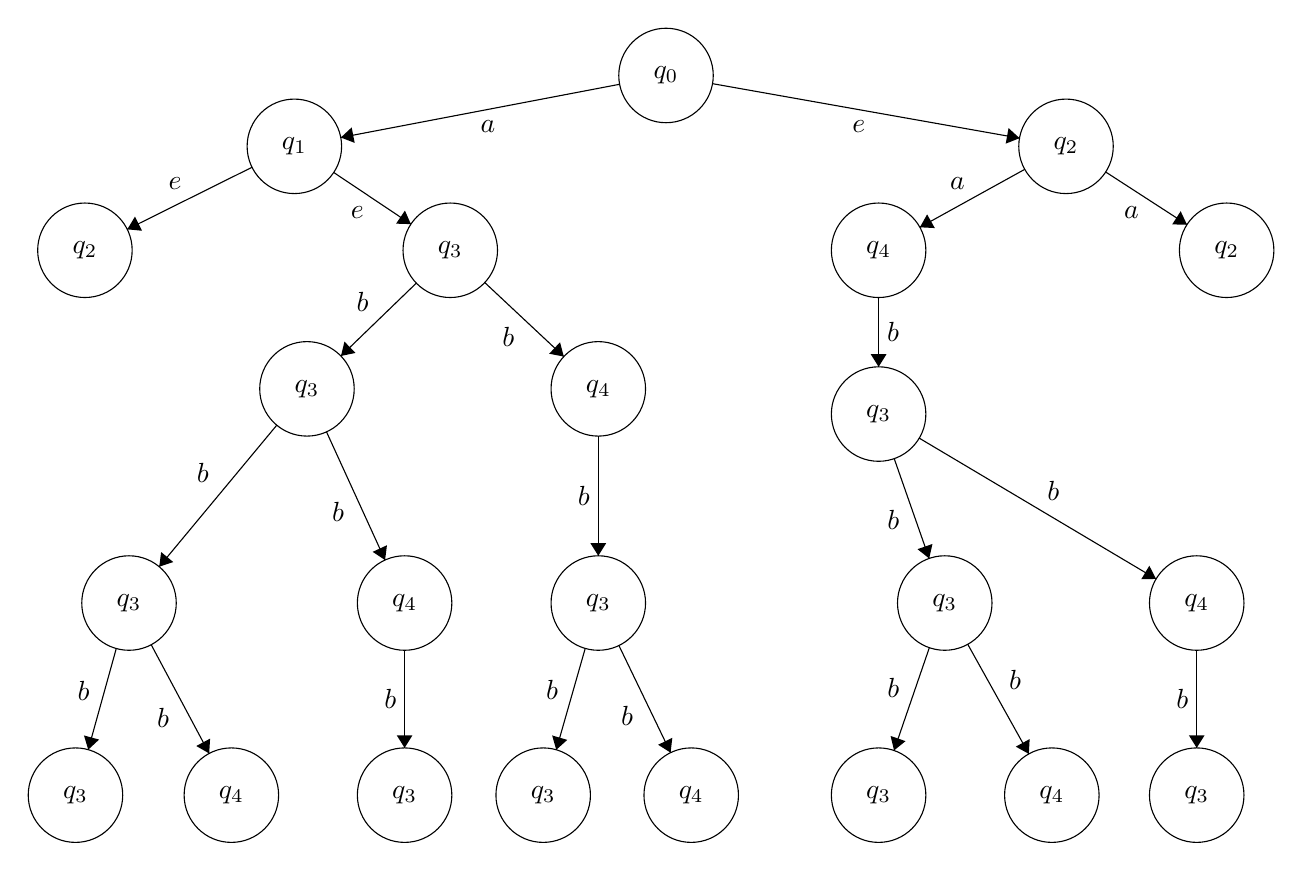
\begin{tikzpicture}[scale=0.2]
\tikzstyle{every node}+=[inner sep=0pt]
\draw [black] (40.7,-3.4) circle (3);
\draw (40.7,-3.4) node {$q_0$};
\draw [black] (17.1,-7.9) circle (3);
\draw (17.1,-7.9) node {$q_1$};
\draw [black] (66.1,-7.9) circle (3);
\draw (66.1,-7.9) node {$q_2$};
\draw [black] (3.8,-14.5) circle (3);
\draw (3.8,-14.5) node {$q_2$};
\draw [black] (27,-14.5) circle (3);
\draw (27,-14.5) node {$q_3$};
\draw [black] (76.3,-14.5) circle (3);
\draw (76.3,-14.5) node {$q_2$};
\draw [black] (54.2,-14.5) circle (3);
\draw (54.2,-14.5) node {$q_4$};
\draw [black] (17.9,-23.3) circle (3);
\draw (17.9,-23.3) node {$q_3$};
\draw [black] (36.4,-23.3) circle (3);
\draw (36.4,-23.3) node {$q_4$};
\draw [black] (36.4,-36.9) circle (3);
\draw (36.4,-36.9) node {$q_3$};
\draw [black] (6.6,-36.9) circle (3);
\draw (6.6,-36.9) node {$q_3$};
\draw [black] (3.2,-49.1) circle (3);
\draw (3.2,-49.1) node {$q_3$};
\draw [black] (13.1,-49.1) circle (3);
\draw (13.1,-49.1) node {$q_4$};
\draw [black] (32.9,-49.1) circle (3);
\draw (32.9,-49.1) node {$q_3$};
\draw [black] (42.3,-49.1) circle (3);
\draw (42.3,-49.1) node {$q_4$};
\draw [black] (54.2,-24.9) circle (3);
\draw (54.2,-24.9) node {$q_3$};
\draw [black] (58.4,-36.9) circle (3);
\draw (58.4,-36.9) node {$q_3$};
\draw [black] (74.4,-36.9) circle (3);
\draw (74.4,-36.9) node {$q_4$};
\draw [black] (74.4,-49.1) circle (3);
\draw (74.4,-49.1) node {$q_3$};
\draw [black] (54.2,-49.1) circle (3);
\draw (54.2,-49.1) node {$q_3$};
\draw [black] (65.2,-49.1) circle (3);
\draw (65.2,-49.1) node {$q_4$};
\draw [black] (24.1,-36.9) circle (3);
\draw (24.1,-36.9) node {$q_4$};
\draw [black] (24.1,-49.1) circle (3);
\draw (24.1,-49.1) node {$q_3$};
\draw [black] (37.75,-3.96) -- (20.05,-7.34);
\fill [black] (20.05,-7.34) -- (20.93,-7.68) -- (20.74,-6.7);
\draw (29.4,-6.24) node [below] {$a$};
\draw [black] (43.65,-3.92) -- (63.15,-7.38);
\fill [black] (63.15,-7.38) -- (62.45,-6.74) -- (62.27,-7.73);
\draw (52.95,-6.24) node [below] {$e$};
\draw [black] (14.41,-9.23) -- (6.49,-13.17);
\fill [black] (6.49,-13.17) -- (7.43,-13.26) -- (6.98,-12.36);
\draw (9.52,-10.7) node [above] {$e$};
\draw [black] (19.6,-9.56) -- (24.5,-12.84);
\fill [black] (24.5,-12.84) -- (24.12,-11.98) -- (23.56,-12.81);
\draw (21.1,-11.7) node [below] {$e$};
\draw [black] (29.19,-16.55) -- (34.21,-21.25);
\fill [black] (34.21,-21.25) -- (33.97,-20.34) -- (33.28,-21.07);
\draw (30.68,-19.38) node [below] {$b$};
\draw [black] (24.84,-16.59) -- (20.06,-21.21);
\fill [black] (20.06,-21.21) -- (20.98,-21.02) -- (20.28,-20.3);
\draw (21.43,-18.42) node [above] {$b$};
\draw [black] (15.98,-25.61) -- (8.52,-34.59);
\fill [black] (8.52,-34.59) -- (9.41,-34.3) -- (8.64,-33.66);
\draw (11.7,-28.66) node [left] {$b$};
\draw [black] (5.79,-39.79) -- (4.01,-46.21);
\fill [black] (4.01,-46.21) -- (4.7,-45.57) -- (3.74,-45.31);
\draw (4.13,-42.46) node [left] {$b$};
\draw [black] (8.01,-39.55) -- (11.69,-46.45);
\fill [black] (11.69,-46.45) -- (11.75,-45.51) -- (10.87,-45.98);
\draw (9.17,-44.17) node [left] {$b$};
\draw [black] (35.57,-39.78) -- (33.73,-46.22);
\fill [black] (33.73,-46.22) -- (34.43,-45.59) -- (33.47,-45.31);
\draw (33.88,-42.43) node [left] {$b$};
\draw [black] (37.71,-39.6) -- (40.99,-46.4);
\fill [black] (40.99,-46.4) -- (41.1,-45.46) -- (40.2,-45.9);
\draw (38.64,-44.07) node [left] {$b$};
\draw [black] (36.4,-26.3) -- (36.4,-33.9);
\fill [black] (36.4,-33.9) -- (36.9,-33.1) -- (35.9,-33.1);
\draw (35.9,-30.1) node [left] {$b$};
\draw [black] (54.2,-17.5) -- (54.2,-21.9);
\fill [black] (54.2,-21.9) -- (54.7,-21.1) -- (53.7,-21.1);
\draw (54.7,-19.7) node [right] {$b$};
\draw [black] (55.19,-27.73) -- (57.41,-34.07);
\fill [black] (57.41,-34.07) -- (57.62,-33.15) -- (56.67,-33.48);
\draw (55.54,-31.65) node [left] {$b$};
\draw [black] (56.78,-26.43) -- (71.82,-35.37);
\fill [black] (71.82,-35.37) -- (71.39,-34.53) -- (70.88,-35.39);
\draw (65.3,-30.4) node [above] {$b$};
\draw [black] (74.4,-39.9) -- (74.4,-46.1);
\fill [black] (74.4,-46.1) -- (74.9,-45.3) -- (73.9,-45.3);
\draw (73.9,-43) node [left] {$b$};
\draw [black] (57.42,-39.74) -- (55.18,-46.26);
\fill [black] (55.18,-46.26) -- (55.91,-45.67) -- (54.96,-45.34);
\draw (55.54,-42.27) node [left] {$b$};
\draw [black] (59.86,-39.52) -- (63.74,-46.48);
\fill [black] (63.74,-46.48) -- (63.79,-45.54) -- (62.91,-46.02);
\draw (62.46,-41.8) node [right] {$b$};
\draw [black] (63.48,-9.36) -- (56.82,-13.04);
\fill [black] (56.82,-13.04) -- (57.77,-13.09) -- (57.28,-12.22);
\draw (59.21,-10.7) node [above] {$a$};
\draw [black] (68.62,-9.53) -- (73.78,-12.87);
\fill [black] (73.78,-12.87) -- (73.38,-12.02) -- (72.84,-12.86);
\draw (70.26,-11.7) node [below] {$a$};
\draw [black] (19.14,-26.03) -- (22.86,-34.17);
\fill [black] (22.86,-34.17) -- (22.98,-33.23) -- (22.07,-33.65);
\draw (20.28,-31.12) node [left] {$b$};
\draw [black] (24.1,-39.9) -- (24.1,-46.1);
\fill [black] (24.1,-46.1) -- (24.6,-45.3) -- (23.6,-45.3);
\draw (23.6,-43) node [left] {$b$};
\end{tikzpicture}
\end{center}

Looking at this computation tree which represent all the possible paths following $w_1=abbb$. The leaf nodes represent the states that we can possibly reach and the states that there is no corresponding way for the current symbol $\sigma \in \Sigma$, meaning $w_1=\sigma w_1'$. Since none of the leaf nodes is $q_5$ which is the only final state. There does not exist a possible path that $(q_0,w_1)\vdash _M^* (q_5,e)$ would be true. So $w_1$ is not in this language.
\subsection*{b.}

\begin{equation} 
\begin{split}
(q_0,ababa)  & \vdash_M (q_1,baba) \\
& \vdash_M (q_3,baba) \\
& \vdash_M (q_3,aba) \\
& \vdash_M (q_1,ba) \\
& \vdash_M (q_3,ba) \\
& \vdash_M (q_3,a) \\
& \vdash_M (q_5,e) 
\end{split}
\end{equation} 
$q_5\in F$, therefore $w_2\in L(N)$.


\section*{Answer 4}

\subsection*{a.}
$N_G=(K_G,\Sigma _G,s_G,\Delta _G,F_G)$ where
$$K_G=K\cup \{q_4,q_5\} =\{q_0,q_1,q_2,q_3,q_4,q_5\}, s_G=q_4,F_G=\{q_5\}$$ 
$$\Sigma _G=\Sigma \cup R_0\ (\ R_0\ \text{is a finite subset of }R\ \text{over }\Sigma)$$
$\Delta _G=\{(q_0, b, q_1),
(q_1, a, q_2), (q_1, e, q_3),
(q_2, a, q_0), (q_2, b, q_1), (q_2, b, q_2), (q_2, b, q_3), (q_3, b, q_1), (q_3, a, q_3)\\ ,
 (q_4,e,q_0), (q_2,e,q_5), (q_3,e,q_5)\}$ \\ \\
The diagram of $N_G \approx N:$
\begin{center}
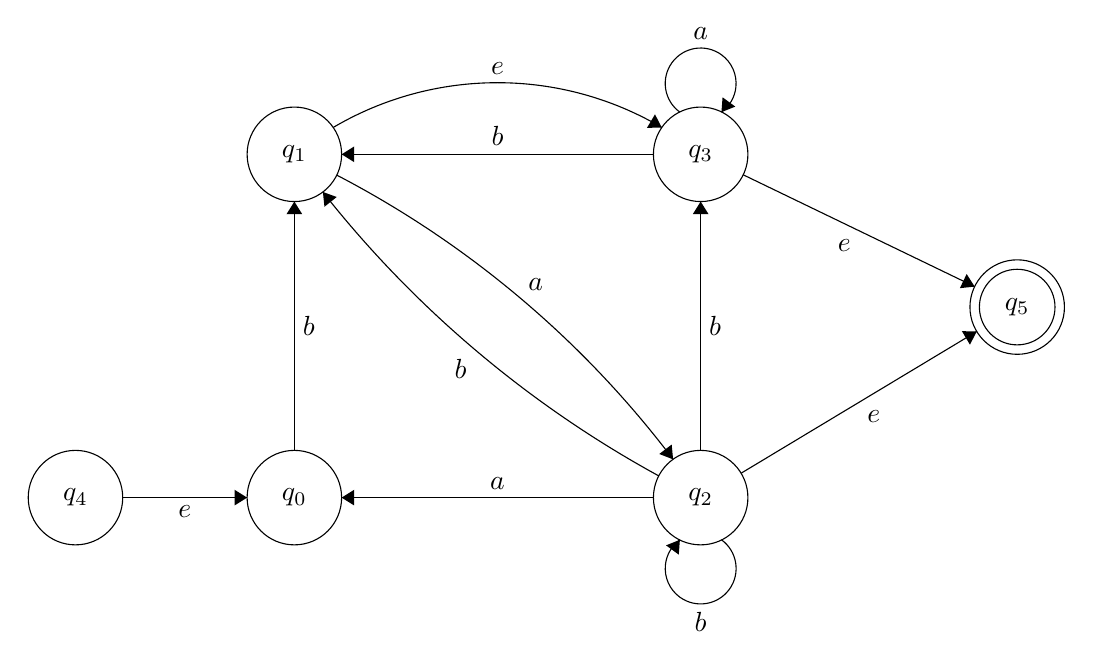
\begin{tikzpicture}[scale=0.2]
\tikzstyle{every node}+=[inner sep=0pt]
\draw [black] (18.1,-31.3) circle (3);
\draw (18.1,-31.3) node {$q_0$};
\draw [black] (18.1,-9.5) circle (3);
\draw (18.1,-9.5) node {$q_1$};
\draw [black] (43.9,-31.3) circle (3);
\draw (43.9,-31.3) node {$q_2$};
\draw [black] (43.9,-9.5) circle (3);
\draw (43.9,-9.5) node {$q_3$};
\draw [black] (4.2,-31.3) circle (3);
\draw (4.2,-31.3) node {$q_4$};
\draw [black] (64,-19.2) circle (2.4);
\draw [black] (64,-19.2) circle (3);
\draw (64,-19.2) node {$q_5$};
\draw [black] (18.1,-28.3) -- (18.1,-12.5);
\fill [black] (18.1,-12.5) -- (17.6,-13.3) -- (18.6,-13.3);
\draw (18.6,-20.4) node [right] {$b$};
\draw [black] (20.793,-10.821) arc (62.51225:37.09472:63.54);
\fill [black] (42.15,-28.87) -- (42.06,-27.93) -- (41.27,-28.53);
\draw (33.43,-18.16) node [above] {$a$};
\draw [black] (20.565,-7.795) arc (120.48728:59.51272:20.567);
\fill [black] (41.43,-7.8) -- (41,-6.96) -- (40.49,-7.82);
\draw (31,-4.45) node [above] {$e$};
\draw [black] (40.9,-31.3) -- (21.1,-31.3);
\fill [black] (21.1,-31.3) -- (21.9,-31.8) -- (21.9,-30.8);
\draw (31,-30.8) node [above] {$a$};
\draw [black] (41.237,-29.918) arc (-118.65782:-141.73521:69.804);
\fill [black] (19.91,-11.89) -- (20.01,-12.83) -- (20.79,-12.21);
\draw (28.65,-22.48) node [below] {$b$};
\draw [black] (45.223,-33.98) arc (54:-234:2.25);
\draw (43.9,-38.55) node [below] {$b$};
\fill [black] (42.58,-33.98) -- (41.7,-34.33) -- (42.51,-34.92);
\draw [black] (43.9,-28.3) -- (43.9,-12.5);
\fill [black] (43.9,-12.5) -- (43.4,-13.3) -- (44.4,-13.3);
\draw (44.4,-20.4) node [right] {$b$};
\draw [black] (40.9,-9.5) -- (21.1,-9.5);
\fill [black] (21.1,-9.5) -- (21.9,-10) -- (21.9,-9);
\draw (31,-9) node [above] {$b$};
\draw [black] (42.577,-6.82) arc (234:-54:2.25);
\draw (43.9,-2.25) node [above] {$a$};
\fill [black] (45.22,-6.82) -- (46.1,-6.47) -- (45.29,-5.88);
\draw [black] (46.6,-10.8) -- (61.3,-17.9);
\fill [black] (61.3,-17.9) -- (60.79,-17.1) -- (60.36,-18);
\draw (53.02,-14.86) node [below] {$e$};
\draw [black] (46.47,-29.75) -- (61.43,-20.75);
\fill [black] (61.43,-20.75) -- (60.49,-20.73) -- (61,-21.59);
\draw (54.89,-25.75) node [below] {$e$};
\draw [black] (7.2,-31.3) -- (15.1,-31.3);
\fill [black] (15.1,-31.3) -- (14.3,-30.8) -- (14.3,-31.8);
\draw (11.15,-31.8) node [below] {$e$};
\end{tikzpicture}
\end{center}

\subsection*{b.}
$R(i,j,k)=R(i,j,k-1)\cup R(i,k,k-1)R(k,k,k-1)^*R(k,j,k-1)$. Using this recursive formula we can do state eliminations by building four generalized state machines as the following way \\ \\ 
$R(4,5,5)=R(4,5,4)\cup R(4,5,4)R(5,5,4)^*R(5,5,4)$ \\
$R(4,5,4)=R(4,5,3)\cup R(4,4,3)R(4,4,3)^*R(4,5,3)$ \\
$R(4,5,3)=R(4,5,2)\cup R(4,3,2)R(3,3,2)^*R(3,5,2)$ \\
$R(4,5,2)=R(4,5,1)\cup R(4,2,1)R(2,2,1)^*R(2,5,1)$ \\
$R(4,5,1)=R(4,5,0)\cup R(4,1,0)R(1,1,0)^*R(1,5,0)$ \\
$R(4,5,1)=R(4,5,0)=R(4,1,0)=R(1,1,0)=R(1,5,0)=\{e\}$ \\ \\ \\ \par
We construct $N_{G_1}\approx N_G \approx N$ by elimination of $q_0$\\
The diagram of $N_{G_1}:$
\begin{center}
\begin{tikzpicture}[scale=0.2]
\tikzstyle{every node}+=[inner sep=0pt]
\draw [black] (18.1,-9.5) circle (3);
\draw (18.1,-9.5) node {$q_1$};
\draw [black] (43.9,-31.3) circle (3);
\draw (43.9,-31.3) node {$q_2$};
\draw [black] (43.9,-9.5) circle (3);
\draw (43.9,-9.5) node {$q_3$};
\draw [black] (4.2,-31.3) circle (3);
\draw (4.2,-31.3) node {$q_4$};
\draw [black] (64,-19.2) circle (2.4);
\draw [black] (64,-19.2) circle (3);
\draw (64,-19.2) node {$q_5$};
\draw [black] (20.793,-10.821) arc (62.51225:37.09472:63.54);
\fill [black] (42.15,-28.87) -- (42.06,-27.93) -- (41.27,-28.53);
\draw (33.43,-18.16) node [above] {$a$};
\draw [black] (20.565,-7.795) arc (120.48728:59.51272:20.567);
\fill [black] (41.43,-7.8) -- (41,-6.96) -- (40.49,-7.82);
\draw (31,-4.45) node [above] {$e$};
\draw [black] (41.187,-30.021) arc (-116.6812:-143.71183:59.863);
\fill [black] (19.81,-11.96) -- (19.88,-12.9) -- (20.69,-12.31);
\draw (26.51,-22.75) node [below] {$bUba$};
\draw [black] (45.223,-33.98) arc (54:-234:2.25);
\draw (43.9,-38.55) node [below] {$b$};
\fill [black] (42.58,-33.98) -- (41.7,-34.33) -- (42.51,-34.92);
\draw [black] (43.9,-28.3) -- (43.9,-12.5);
\fill [black] (43.9,-12.5) -- (43.4,-13.3) -- (44.4,-13.3);
\draw (44.4,-20.4) node [right] {$b$};
\draw [black] (40.9,-9.5) -- (21.1,-9.5);
\fill [black] (21.1,-9.5) -- (21.9,-10) -- (21.9,-9);
\draw (31,-9) node [above] {$b$};
\draw [black] (42.577,-6.82) arc (234:-54:2.25);
\draw (43.9,-2.25) node [above] {$a$};
\fill [black] (45.22,-6.82) -- (46.1,-6.47) -- (45.29,-5.88);
\draw [black] (46.6,-10.8) -- (61.3,-17.9);
\fill [black] (61.3,-17.9) -- (60.79,-17.1) -- (60.36,-18);
\draw (53.02,-14.86) node [below] {$e$};
\draw [black] (46.47,-29.75) -- (61.43,-20.75);
\fill [black] (61.43,-20.75) -- (60.49,-20.73) -- (61,-21.59);
\draw (54.89,-25.75) node [below] {$e$};
\draw [black] (5.81,-28.77) -- (16.49,-12.03);
\fill [black] (16.49,-12.03) -- (15.64,-12.44) -- (16.48,-12.97);
\draw (11.77,-21.71) node [right] {$b$};
\end{tikzpicture}
\end{center} \par
We construct $N_{G_2}\approx N_{G_1}$ by elimination of $q_1$\\
The diagram of $N_{G_2}:$
\begin{center}
\begin{tikzpicture}[scale=0.2]
\tikzstyle{every node}+=[inner sep=0pt]
\draw [black] (43.9,-31.3) circle (3);
\draw (43.9,-31.3) node {$q_2$};
\draw [black] (43.9,-9.5) circle (3);
\draw (43.9,-9.5) node {$q_3$};
\draw [black] (4.2,-31.3) circle (3);
\draw (4.2,-31.3) node {$q_4$};
\draw [black] (64,-19.2) circle (2.4);
\draw [black] (64,-19.2) circle (3);
\draw (64,-19.2) node {$q_5$};
\draw [black] (45.223,-33.98) arc (54:-234:2.25);
\draw (43.9,-38.55) node [below] {$b\cup ba\cup aba$};
\fill [black] (42.58,-33.98) -- (41.7,-34.33) -- (42.51,-34.92);
\draw [black] (44.988,-12.294) arc (18.00196:-18.00196:26.229);
\fill [black] (44.99,-12.29) -- (44.76,-13.21) -- (45.71,-12.9);
\draw (46.77,-20.4) node [right] {$b\cup ab$};
\draw [black] (42.577,-6.82) arc (234:-54:2.25);
\draw (43.9,-2.25) node [above] {$a\cup b$};
\fill [black] (45.22,-6.82) -- (46.1,-6.47) -- (45.29,-5.88);
\draw [black] (46.6,-10.8) -- (61.3,-17.9);
\fill [black] (61.3,-17.9) -- (60.79,-17.1) -- (60.36,-18);
\draw (53.02,-14.86) node [below] {$e$};
\draw [black] (46.47,-29.75) -- (61.43,-20.75);
\fill [black] (61.43,-20.75) -- (60.49,-20.73) -- (61,-21.59);
\draw (54.89,-25.75) node [below] {$e$};
\draw [black] (7.2,-31.3) -- (40.9,-31.3);
\fill [black] (40.9,-31.3) -- (40.1,-30.8) -- (40.1,-31.8);
\draw (24.05,-31.8) node [below] {$ba$};
\draw [black] (6.83,-29.86) -- (41.27,-10.94);
\fill [black] (41.27,-10.94) -- (40.33,-10.89) -- (40.81,-11.77);
\draw (23.05,-19.9) node [above] {$b$};
\draw [black] (43.018,-28.434) arc (-165.55483:-194.44517:32.206);
\fill [black] (43.02,-28.43) -- (43.3,-27.53) -- (42.33,-27.78);
\draw (41.5,-20.4) node [left] {$ba$};
\end{tikzpicture}
\end{center} 
\vspace{4cm} \par
We construct $N_{G_3}\approx N_{G_2}$ by elimination of $q_2$\\
The diagram of $N_{G_3}:$
\begin{center}
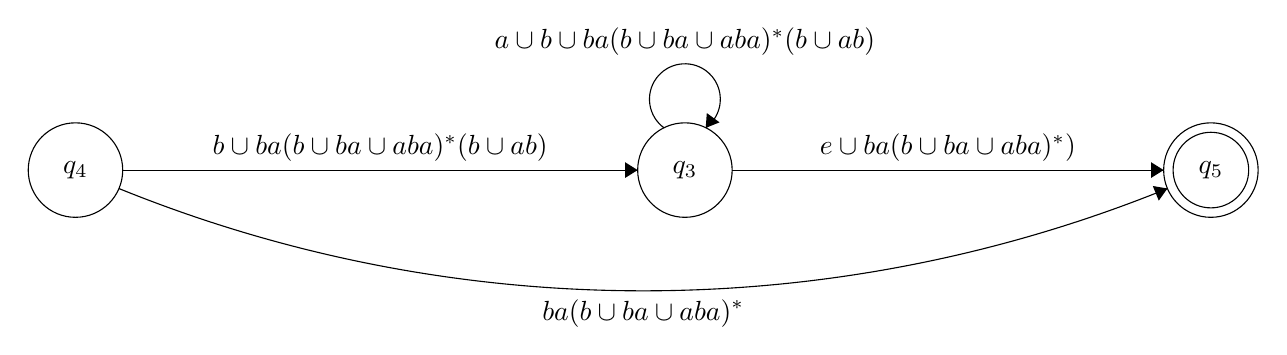
\begin{tikzpicture}[scale=0.2]
\tikzstyle{every node}+=[inner sep=0pt]
\draw [black] (42.9,-31.3) circle (3);
\draw (42.9,-31.3) node {$q_3$};
\draw [black] (4.2,-31.3) circle (3);
\draw (4.2,-31.3) node {$q_4$};
\draw [black] (76.3,-31.3) circle (2.4);
\draw [black] (76.3,-31.3) circle (3);
\draw (76.3,-31.3) node {$q_5$};
\draw [black] (41.577,-28.62) arc (234:-54:2.25);
\draw (42.9,-24.05) node [above] {$a\cup b\cup ba(b\cup ba\cup aba)^*(b\cup ab)$};
\fill [black] (44.22,-28.62) -- (45.1,-28.27) -- (44.29,-27.68);
\draw [black] (45.9,-31.3) -- (73.3,-31.3);
\fill [black] (73.3,-31.3) -- (72.5,-30.8) -- (72.5,-31.8);
\draw (59.6,-30.8) node [above] {$e\cup ba(b\cup ba\cup aba)^*)$};
\draw [black] (7.2,-31.3) -- (39.9,-31.3);
\fill [black] (39.9,-31.3) -- (39.1,-30.8) -- (39.1,-31.8);
\draw (23.55,-30.8) node [above] {$b\cup ba(b\cup ba\cup aba)^*(b\cup ab)$};
\draw [black] (73.54,-32.475) arc (-67.91976:-112.08024:88.559);
\fill [black] (73.54,-32.47) -- (72.61,-32.31) -- (72.99,-33.24);
\draw (40.25,-39.47) node [below] {$ba(b\cup ba\cup aba)^*$};
\end{tikzpicture}
\end{center} \par
We construct $N_{G_4}\approx N_{G_3}$ by elimination of $q_3$\\
The diagram of $N_{G_4}:$
\begin{center}
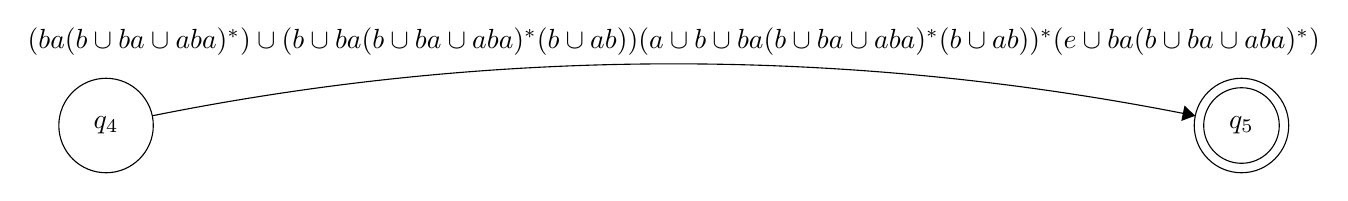
\begin{tikzpicture}[scale=0.2]
\tikzstyle{every node}+=[inner sep=0pt]
\draw [black] (4.2,-31.3) circle (3);
\draw (4.2,-31.3) node {$q_4$};
\draw [black] (76.3,-31.3) circle (2.4);
\draw [black] (76.3,-31.3) circle (3);
\draw (76.3,-31.3) node {$q_5$};
\draw [black] (7.136,-30.682) arc (101.38508:78.61492:167.751);
\fill [black] (73.36,-30.68) -- (72.68,-30.03) -- (72.48,-31.01);
\draw (40.25,-26.88) node [above] {$(ba(b\cup ba\cup aba)^*)\cup (b\cup ba(b\cup ba\cup aba)^*(b\cup ab))(a\cup b\cup ba(b\cup ba\cup aba)^*(b\cup ab))^*(e\cup ba(b\cup ba\cup aba)^*)$};
\end{tikzpicture}
\end{center} \par
$L(N_{G_4})=L(N)=\\
(ba(b\cup ba\cup aba)^*)\cup (b\cup ba(b\cup ba\cup aba)^*(b\cup ab))(a\cup b\cup ba(b\cup ba\cup aba)^*(b\cup ab))^*(e\cup ba(b\cup ba\cup aba)^*)$


\section*{Answer 5}

\subsection*{a.}

We are given that NFA $N=(K,\Sigma,\Delta,q_0,F)$. Define DFA $M$ as $M=(K',\Sigma,\delta ',s',F')$. \\
Before we covert NFA $N$ to equivalent DFA $M$. We need to give some general definitions that we are going to use,
\begin{equation} 
\begin{split}
E(q) & = \{ p\in K:\ (q,e)\vdash _N^*(p,e)\} \\
\delta '(Q,a) & = \bigcup \{ E(p):\ p\in K\ and\ (q,a,p)\in \Delta\ for\ some\ q\in Q,\ a\in \Sigma \} \\
(q,w)& \vdash_N^*(p,e)\ if\ and\ only\ if\ (E(q),w)\vdash _M^*(P,e)\ \ for\ some\ set\ P\ containing\ p
\end{split}
\end{equation} 
We have defined $E(q)$ for each state $q$ of $N$. So, $$s'=E(q_0)=\{q_0,q_1,q_2\}$$
\quad \qquad \qquad \qquad $(q_0,a,q_1),\ (q_2,a,q_3)$ are all the transtitons $(q,a,p)$ for some $q\in s'$. So, 
$$\delta '(s',a)=E(q_1)\cup E(q_3)=\{q_1,q_3\}$$
\quad \qquad \qquad \qquad $(q_0,b,q_2)$ is the only transtiton $(q,a,p)$ for some $q\in s'$. So, 
$$\delta '(s',b)=E(q_2)=\{q_2\}$$
Repeating this calculation for newly introduced states, we have the following.
\begin{equation} 
\begin{split}
\delta '(\{q_1,q_3\},a) & = \emptyset \\
\delta '(\{q_1,q_3\},b) & = E(q_1) = \{q_1\} \\
\delta '(\{q_2\},a) & = E(q_3) =  \{q_1,q_3\} \\
\delta '(\{q_2\},b) & = \emptyset \\
\delta '(\{ \emptyset \},a) & = \delta '(\{ \emptyset \},b) = \emptyset \\
\delta '(\{q_1\},a) & = \delta '(\{q_1\},b) = \emptyset 
\end{split}
\end{equation} 
Now we can conclude relevant states for $K'$, since there would have been $2^4=16$ states it is not convenient to declare all possible states before $\delta '$. $K'=\{ \{q_0,q_1,q_2\}, \{q_1,q_3\}, \{q_2 \}, \{q_1\}, \emptyset \}$. \\
$F'=\{Q\subseteq K:\ Q\cap F \neq \emptyset \}$. $F'$, the set of final states, contains each set of states which $q_3$ is a member of. Since $q_3$ is the only member of $F$. Meaning, So, $F'=\{q_1,q_3\}$ \\
The illustration of the transition state function, $\delta '$, is the following. \\ \\
\textbf{\underline{Start state}: }$\{q_0,q_1,q_2\}$
\begin{center}
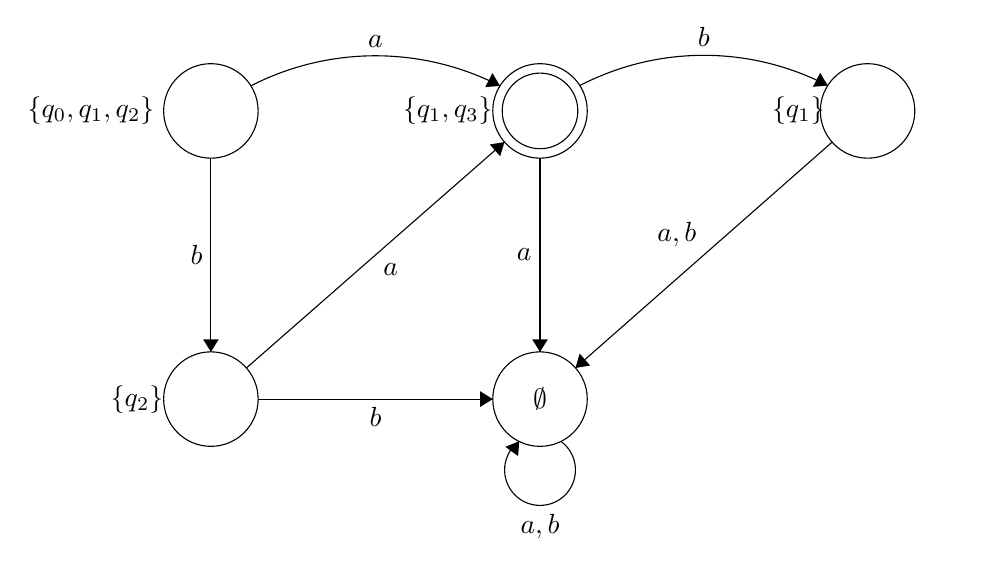
\begin{tikzpicture}[scale=0.2]
\tikzstyle{every node}+=[inner sep=0pt]
\draw [black] (18.8,-19.2) circle (3);
\draw (18.8,-19.2) node {${\{q_0,q_1,q_2\}}\mbox{ }\mbox{ }\mbox{ }\mbox{ }\mbox{ }\mbox{ }\mbox{ }\mbox{ }\mbox{ }\mbox{ }\mbox{ }\mbox{ }\mbox{ }\mbox{ }\mbox{ }\mbox{ }\mbox{ }\mbox{ }\mbox{ }\mbox{ }\mbox{ }\mbox{ }\mbox{ }\mbox{ }\mbox{ }\mbox{ }$};
\draw [black] (39.7,-19.2) circle (3);
\draw (39.7,-19.2) node {${\{q_1,q_3\}}\mbox{ }\mbox{ }\mbox{ }\mbox{ }\mbox{ }\mbox{ }\mbox{ }\mbox{ }\mbox{ }\mbox{ }\mbox{ }\mbox{ }\mbox{ }\mbox{ }\mbox{ }\mbox{ }\mbox{ }\mbox{ }\mbox{ }\mbox{ }$};
\draw [black] (39.7,-19.2) circle (2.4);
\draw [black] (18.8,-37.5) circle (3);
\draw (18.8,-37.5) node {${\{q_2}\}\mbox{ }\mbox{ }\mbox{ }\mbox{ }\mbox{ }\mbox{ }\mbox{ }\mbox{ }\mbox{ }\mbox{ }\mbox{ }\mbox{ }\mbox{ }\mbox{ }\mbox{ }\mbox{ }$};
\draw [black] (39.7,-37.5) circle (3);
\draw (39.7,-37.5) node {$\emptyset$};
\draw [black] (60.5,-19.2) circle (3);
\draw (60.5,-19.2) node {${\{q_1\}}\mbox{ }\mbox{ }\mbox{ }\mbox{ }\mbox{ }\mbox{ }\mbox{ }\mbox{ }\mbox{ }\mbox{ }\mbox{ }\mbox{ }\mbox{ }\mbox{ }\mbox{ }$};
\draw [black] (18.8,-22.2) -- (18.8,-34.5);
\fill [black] (18.8,-34.5) -- (19.3,-33.7) -- (18.3,-33.7);
\draw (18.3,-28.35) node [left] {$b$};
\draw [black] (21.8,-37.5) -- (36.7,-37.5);
\fill [black] (36.7,-37.5) -- (35.9,-37) -- (35.9,-38);
\draw (29.25,-38) node [below] {$b$};
\draw [black] (39.7,-22.2) -- (39.7,-34.5);
\fill [black] (39.7,-34.5) -- (40.2,-33.7) -- (39.2,-33.7);
\draw (39.2,-28.35) node [left] {$a$};
\draw [black] (21.06,-35.52) -- (37.44,-21.18);
\fill [black] (37.44,-21.18) -- (36.51,-21.33) -- (37.17,-22.08);
\draw (30.21,-28.84) node [below] {$a$};
\draw [black] (21.338,-17.608) arc (117.14115:62.85885:17.343);
\fill [black] (37.16,-17.61) -- (36.68,-16.8) -- (36.22,-17.69);
\draw (29.25,-15.2) node [above] {$a$};
\draw [black] (58.25,-21.18) -- (41.95,-35.52);
\fill [black] (41.95,-35.52) -- (42.88,-35.37) -- (42.22,-34.61);
\draw (48.39,-27.86) node [above] {$a,b$};
\draw [black] (42.228,-17.591) arc (117.4442:62.5558:17.081);
\fill [black] (57.97,-17.59) -- (57.49,-16.78) -- (57.03,-17.67);
\draw (50.1,-15.17) node [above] {$b$};
\draw [black] (41.023,-40.18) arc (54:-234:2.25);
\draw (39.7,-44.75) node [below] {$a,b$};
\fill [black] (38.38,-40.18) -- (37.5,-40.53) -- (38.31,-41.12);
\end{tikzpicture}
\end{center}
\vspace{8cm}
\subsection*{b.}
L=\{a,ba\}. The complement of the language $L$ can expressed as $\overline{L}=\{a,b\}^*-L$ \\
$\overline{L}=L(M)$ such that \par
$M=(K=\{q_0,q_1,q_2,q_3\},\ \Sigma = \{a,b\},\ \delta,\ s=q_0,\ F=\{q_0,q_2,q_3\})$ 
$$\text{where } \delta(q_0,a)=q_1,\ \delta(q_0,b)=q_2,\ \delta(q_1,a)=q_4,\ \delta(q_1,b)=q_3$$
$$\delta(q_2,a)=q_1,\ \delta(q_2,b)=q_3,\ \delta(q_3,a)=q_3,\ \delta(q_3,b)=q_3$$

\begin{center}
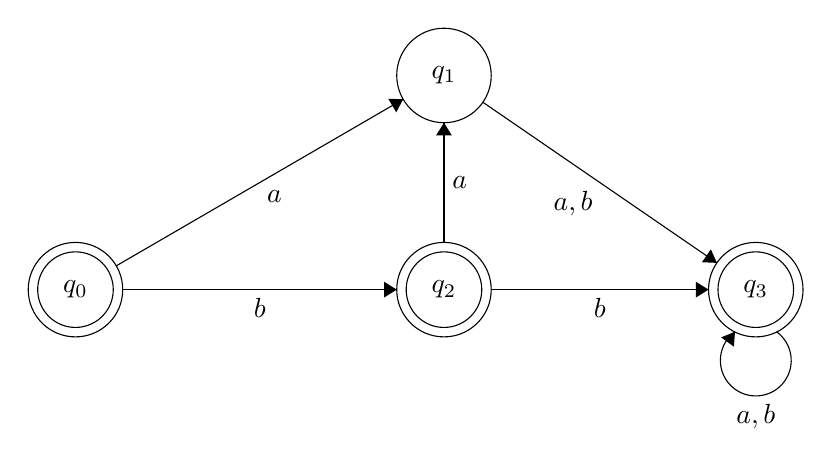
\begin{tikzpicture}[scale=0.2]
\tikzstyle{every node}+=[inner sep=0pt]
\draw [black] (19.7,-19.7) circle (3);
\draw (19.7,-19.7) node {$q_0$};
\draw [black] (19.7,-19.7) circle (2.4);
\draw [black] (43.1,-6.1) circle (3);
\draw (43.1,-6.1) node {$q_1$};
\draw [black] (43.1,-19.7) circle (3);
\draw (43.1,-19.7) node {$q_2$};
\draw [black] (43.1,-19.7) circle (2.4);
\draw [black] (62.9,-19.7) circle (3);
\draw (62.9,-19.7) node {$q_3$};
\draw [black] (62.9,-19.7) circle (2.4);
\draw [black] (22.29,-18.19) -- (40.51,-7.61);
\fill [black] (40.51,-7.61) -- (39.56,-7.58) -- (40.07,-8.44);
\draw (32.34,-13.4) node [below] {$a$};
\draw [black] (22.7,-19.7) -- (40.1,-19.7);
\fill [black] (40.1,-19.7) -- (39.3,-19.2) -- (39.3,-20.2);
\draw (31.4,-20.2) node [below] {$b$};
\draw [black] (46.1,-19.7) -- (59.9,-19.7);
\fill [black] (59.9,-19.7) -- (59.1,-19.2) -- (59.1,-20.2);
\draw (53,-20.2) node [below] {$b$};
\draw [black] (64.223,-22.38) arc (54:-234:2.25);
\draw (62.9,-26.95) node [below] {$a,b$};
\fill [black] (61.58,-22.38) -- (60.7,-22.73) -- (61.51,-23.32);
\draw [black] (45.57,-7.8) -- (60.43,-18);
\fill [black] (60.43,-18) -- (60.05,-17.14) -- (59.48,-17.96);
\draw (51.3,-13.4) node [below] {$a,b$};
\draw [black] (43.1,-16.7) -- (43.1,-9.1);
\fill [black] (43.1,-9.1) -- (42.6,-9.9) -- (43.6,-9.9);
\draw (43.6,-12.9) node [right] {$a$};
\end{tikzpicture}
\end{center}
$$\overline{L}=\emptyset \cup b\cup (aa\cup ab\cup bb\cup baa\cup bab)a^*b^*$$
$$\overline{L}=\{w\in \Sigma ^*:\ w\neq a\ and\ w\neq ba \}$$

\section*{Answer 6}
Given two regular languages $L_1,L_2$ and nondeterministic automata $M_1$, $M_2$ such that, \\
$L_1=L(M_1),\ L_2=L(M_2)\ where\ M_1=(K_1,\Sigma _1, \Delta _1, s_1, F_1),\ M_2=(K_2,\Sigma _2, \Delta _2, s_2, F_2),\ $ \\
We need to construct $M=M_1 - M_2$ such that $L(M)=L(M_1) - L(M_2)$ as follows
$$M=(K,\Sigma,\Delta,s,F)$$ 
where 
$$\Sigma = \Sigma _1 \cup \Sigma_2,\ K=K_1\text{x} K_2,\ s=(s_1,s_2),\ F=F_1\text{x}(K_2-F_2)$$
and $\Delta$ is defined as follows \\
$$\Delta = \Delta _x \cup \Delta _y \cup \Delta _z$$
$\Delta _x=\{((q_1,q_2),\sigma ,(p_1,p_2)): (q_1,\sigma,p_1)\in \Delta _1\ and\ (q_2,\sigma,p_2)\in \Delta _2, \sigma \in \Sigma \}$ \\
$\Delta _y=\{((q_1,q_2),\sigma ,(p_1,p_2)): \sigma =e,\ (q_1,e,p_1)\in \Delta _1\ and\ q_2=p_2\}$ \\
$\Delta _z=\{((q_1,q_2),\sigma ,(p_1,p_2)): \sigma =e,\ (q_2,e,p_2)\in \Delta _2\ and\ q_1=p_1\}$ \\ \par
If $w\in \Sigma ^*$, then $(s,w)\vdash _M^*(q,e)$ for some $q\in F$ if and only if $(s_1,w)\vdash _{M_1}^*(q_1,e)$ for some $q_1\in F_1$ and $(s_2,w)\vdash _M^*(q_2,e)$ for some $q_2\in (K_2-F_2)$. Hence $M$ accepts $w$ if and only if $M_1$ accepts $w$ and $M_2$ does not accept $w$, and $L(M)=L(M_1)-L(M_2)$.

\section*{Answer 7}

\subsection*{a.}
If the language L were regular, then Pumping Theorem(Lemma) would apply for some integer $1\leq m$. Consider the string $w\in L$ such that given function holds $f(a,w)=n^2$ for some $n\in N$. By the theorem it can be written as $w=xyz$ such that $|xy|\leq m$ and $y\neq e$. We have two cases to consider. Since $y$ cannot be empty, y can include $a$ or not. These are the two cases that we need to elaborate. We will show that in each case the assumption that $xy^nz\in L$ for all $0\leq n$ leads to contradiction. \par
Case 1: $y$ includes $a$. Then we can say that, \\
$$f(a,x)=p,\ f(a,y)=q,\ f(a,z)=r \text{ for some }0\leq p,\ 0<q,\ 0\leq r$$
$$f(b,x)=s,\ f(b,y)=t,\ f(b,z)=w \text{ for some }0\leq s,\ 0\leq t,\ 0\leq w$$
This means $p+q+r+s+t+w=|xyz|$ and since $|xy|\leq m$, $p+q+s+t\leq m$. \\
The condition $xy^nz\in L$ for all $0\leq n$ becomes 
$$p+qn+r=n^2 \text{ for some } n\in N$$
Showing only one string that leads to a contradiction will be enough. Therefore we can simply choose 
$$p=10,\ 0<q,\ r=0,\ 0\leq s,\ 0\leq t,\ 0\leq w,\ n=0$$ 
This leads to $10+0+0=0$ which is a contradiction because $10=0$. \\ \par
Case 2: $y$ includes $b$. Then we can say that, \\
$$f(a,x)=p,\ f(a,y)=q,\ f(a,z)=r \text{ for some }0\leq p,\ 0\leq q,\ 0\leq r$$
$$f(b,x)=s,\ f(b,y)=t,\ f(b,z)=w \text{ for some }0\leq s,\ 0<t,\ 0\leq w$$
This means $p+q+r+s+t+w=|xyz|$ and since $|xy|\leq m$, $p+q+s+t\leq m$. \\
The condition $xy^nz\in L$ for all $0\leq n$ becomes 
$$p+qn+r=n^2 \text{ for some } n\in N$$
Showing only one string that leads to a contradiction will be enough. Therefore we can simply choose 
$$p=100,\ 0\leq q,\ r=0,\ 0\leq s,\ 0\leq t,\ 0\leq w,\ n=0$$
This leads to $100+0+0=0$ which is a contradiction because $100=0$. 

\end{document}

​

